
% slide-3b.tex

\documentclass[dvipdfmx,notheorems,t]{beamer}

\usepackage{docmute}

% settings.tex

\AtBeginSection[]{\frame[t]{\frametitle{目次}
  \tableofcontents[currentsection,hideallsubsections]}}

\AtBeginSubsection[]{\frame[t]{\frametitle{目次}
  \tableofcontents[currentsection,sectionstyle=show/hide,
  currentsubsection,subsectionstyle=show/shaded/hide]}}

\usefonttheme{professionalfonts}
\usetheme{Madrid}

\setbeamercovered{transparent=30} 
% \setbeamertemplate{navigation symbols}{}
\setbeamertemplate{frametitle}[default][left]
\setbeamertemplate{frametitle continuation}{}
\setbeamertemplate{enumerate items}[square]
\setbeamertemplate{caption}[numbered]

\let\oldframe\frame
\renewcommand\frame[1][t,allowdisplaybreaks,allowframebreaks]{\oldframe[#1]}

\addtobeamertemplate{block begin}{\setlength{\abovedisplayskip}{2.5pt}}

\usepackage{bxdpx-beamer}
\usepackage{pxjahyper}
\usepackage{minijs}

\usepackage{amsmath}
\usepackage{amssymb}
\usepackage{amsthm}
\usepackage{bm}
\usepackage{physics}

% Set the path to the figure
\graphicspath{{fig/}}

\usepackage{multirow}

% Add space in the table
\usepackage{cellspace}

% Add space in the table
\setlength\cellspacetoplimit{5pt}
\setlength\cellspacebottomlimit{5pt}

\usepackage{url}

% \hypersetup{
%   colorlinks = true,
%   urlcolor = blue,
%   linkcolor = black,
%   citecolor = green
% }

\DeclareMathOperator*{\argmax}{arg\,max}
\DeclareMathOperator*{\argmin}{arg\,min}
% \DeclareMathOperator{\Tr}{Tr}
% \DeclareMathOperator{\KL}{KL}
\DeclareMathOperator{\diag}{diag}
\DeclareMathOperator{\sgn}{sgn}
\DeclareMathOperator{\adj}{adj}
\DeclareMathOperator{\EOp}{\mathbb{E}}
\DeclareMathOperator{\HOp}{H}
\DeclareMathOperator{\KLOp}{KL}
\DeclareMathOperator{\VarOp}{Var}
\DeclareMathOperator{\CovOp}{Cov}
\newcommand\E[1]{\EOp \left[ #1 \right]}
\newcommand\Entropy[1]{\HOp \left[ #1 \right]}
\newcommand\MutualInfo[1]{I \left( #1 \right)}
\newcommand\KL[2]{\KLOp \left( #1 \parallel #2 \right)}
\newcommand\Var[1]{\VarOp \left[ #1 \right]}
\newcommand\Cov[2]{\CovOp \left( #1, #2 \right)}

\newcommand\BigO[1]{O \left( #1 \right)}
\newcommand\SmallO[1]{o \left( #1 \right)}

\newcommand\Comb[2]{{}_{#1}C_{#2}}

\newcommand{\middlerel}[1]{\mathrel{}\middle#1\mathrel{}}

\usepackage[T1]{fontenc}
\usepackage[utf8]{inputenc}

\setbeamertemplate{theorems}[numbered]
\theoremstyle{definition}
\newtheorem{theorem}{定理}
\newtheorem{definition}{定義}
\newtheorem{proposition}{命題}
\newtheorem{lemma}{補題}
\newtheorem{corollary}{系}
\newtheorem{conjecture}{予想}
\newtheorem*{remark}{Remark}
\renewcommand{\proofname}{}

\renewcommand{\figurename}{図}
\renewcommand{\tablename}{表}

\renewcommand{\kanjifamilydefault}{\gtdefault}



\title{行列輪講: 第3回 行列とベクトルの微分1}
\author{杉浦 圭祐}
\institute[松谷研究室]{慶應義塾大学理工学部情報工学科 松谷研究室}
\date{\today}

% Always use the \displaystyle
\everymath{\displaystyle}

\begin{document}

\linespread{1.1}

\frame{\titlepage}

\section{}

\begin{frame}[t,allowdisplaybreaks,allowframebreaks]{目次}
\tableofcontents
\end{frame}

\section{概要}

\begin{frame}{このスライドの概要}
\begin{itemize}
  \item 行列とベクトルの微分について確認する
  \begin{itemize}
    \item 微分の種類, レイアウト (表記法)
    \item ベクトルのスカラによる微分
    \item スカラのベクトルによる微分
    \item ベクトルのベクトルによる微分
  \end{itemize}
  \item 以下の資料も大変参考になります:
  \begin{itemize}
    \item \url{math.uwaterloo.ca/~hwolkowi/matrixcookbook.pdf}
    \item \url{comp.nus.edu.sg/cs5240/lecture/matrix-differentiation.pdf}
    \item \url{en.wikipedia.org/wiki/Matrix_calculus}
  \end{itemize}
\end{itemize}
\end{frame}

\section{行列, ベクトルの微分の種類, レイアウト}

\begin{frame}{行列, ベクトルの微分の種類}
\begin{itemize}
  \item 以下の6つの組み合わせがある.
\end{itemize}

\begin{table}[h]
  \centering
  \begin{tabular}{ScScScSc} \hline
    & スカラ & ベクトル & 行列 \\ \hline
    スカラ & $\pdv{y}{x}$ & $\pdv{\vb{y}}{x}$ & $\pdv{\vb{Y}}{x}$ \\ \hline
    ベクトル & $\pdv{y}{\vb{x}}$ & $\pdv{\vb{y}}{\vb{x}}$ & \\ \hline
    行列 & $\pdv{y}{\vb{X}}$ \\ \hline
  \end{tabular}
\end{table}

\begin{itemize}
  \item ベクトルの行列による微分, 行列の行列による微分などは, テンソルで表記される.
\end{itemize}
\end{frame}

\begin{frame}{微分のレイアウト}
\begin{itemize}
  \item スカラの場合とは異なり, レイアウトが統一されていない.
  \item 幾つかの流派があり, 人によって異なる (明記されないことが多い).
  \item どのレイアウトによる表記なのかを理解しないと, 混乱の元になる.
\end{itemize}

\begin{itemize}
  \item 以下の2つのレイアウトに大別される ($\vb{x}, \vb{y}$を縦ベクトルとする).
  \item \textcolor{red}{分子レイアウト} (Numerator Layout)
  \begin{itemize}
    \item $\pdv{\vb{y}}{x}$は, \textcolor{red}{縦ベクトル},
    $\pdv{y}{\vb{x}}$は, \textcolor{red}{横ベクトル}
  \end{itemize}
  \item \textcolor{red}{分母レイアウト} (Denominator Layout)
  \begin{itemize}
    \item $\pdv{\vb{y}}{x}$は, \textcolor{red}{横ベクトル},
    $\pdv{y}{\vb{x}}$は, \textcolor{red}{縦ベクトル}
  \end{itemize}

  \item これらを, 混ぜて使うことも多々ある. 優劣はない.
\end{itemize}
\end{frame}

\begin{frame}{スカラによる微分}
\begin{table}[h]
  \centering
  \begin{tabular}{ScSc}
    分子レイアウト & 分母レイアウト \\ \hline
    $\pdv{y}{x}$ & $\pdv{y}{x}$ \\ \hline
    $\pdv{\vb{y}}{x} = \mqty(\pdv{y_1}{x} \\ \vdots \\ \pdv{y_m}{x})$
      & $\pdv{\vb{y}}{x} = \mqty(\pdv{y_1}{x} & \cdots & \pdv{y_m}{x}) \equiv \pdv{\vb{y}^\top}{x} $ \\ \hline
    $\pdv{\vb{Y}}{x} = \mqty(\pdv{y_{11}}{x} & \cdots & \pdv{y_{1n}}{x} \\
      \vdots & \ddots & \vdots \\
      \pdv{y_{m1}}{x} & \cdots & \pdv{y_{mn}}{x})$ & まれ
  \end{tabular}
\end{table}
\end{frame}

\begin{frame}{ベクトルによる微分}
\begin{table}[h]
  \centering
  \begin{tabular}{ScSc}
    分子レイアウト & 分母レイアウト \\ \hline
    $\pdv{y}{\vb{x}} = \mqty(\pdv{y}{x_1} & \cdots & \pdv{y}{x_n}) \equiv \pdv{y}{\vb{x}^\top}$
      & $\pdv{y}{\vb{x}} = \mqty(\pdv{y}{x_1} \\ \vdots \\ \pdv{y}{x_n})$ \\ \hline
    $\pdv{\vb{y}}{\vb{x}} = \mqty(\pdv{y_1}{x_1} & \cdots & \pdv{y_1}{x_n} \\
      \vdots & \ddots & \vdots \\
      \pdv{y_m}{x_1} & \cdots & \pdv{y_m}{x_n})$
      & $\pdv{\vb{y}}{\vb{x}} = \mqty(\pdv{y_1}{x_1} & \cdots & \pdv{y_m}{x_1} \\
      \vdots & \ddots & \vdots \\
      \pdv{y_1}{x_n} & \cdots & \pdv{y_m}{x_n})$ \\
    $\equiv \pdv{\vb{y}}{\vb{x}^\top}$ & $ \equiv \pdv{\vb{y}^\top}{\vb{x}}$
  \end{tabular}
\end{table}
\end{frame}

\begin{frame}{行列による微分}
\begin{table}[h]
  \centering
  \begin{tabular}{ScSc}
    分子レイアウト & 分母レイアウト \\ \hline
    $\pdv{y}{\vb{X}} = \mqty(\pdv{y}{x_{11}} & \cdots & \pdv{y}{x_{m1}} \\
      \vdots & \ddots & \vdots \\
      \pdv{y}{x_{1n}} & \cdots & \pdv{y}{x_{mn}})$
      & $\pdv{y}{\vb{X}} = \mqty(\pdv{y}{x_{11}} & \cdots & \pdv{y}{x_{1n}} \\
        \vdots & \ddots & \vdots \\
        \pdv{y}{x_{m1}} & \cdots & \pdv{y}{x_{mn}})$ \\
      $\equiv \pdv{y}{\vb{X}^\top}$ & $\equiv \pdv{y}{\vb{X}}$
  \end{tabular}
\end{table}
\end{frame}

\begin{frame}{微分の結果の形}
\begin{figure}
  \centering
  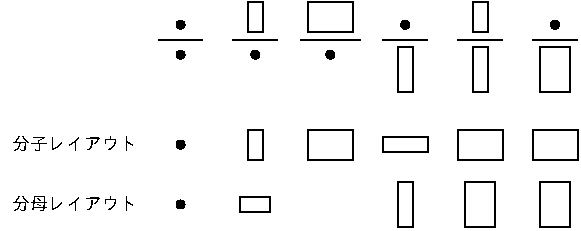
\includegraphics[keepaspectratio, width=0.9\linewidth]{matrix-derivative.pdf}
\end{figure}

\begin{itemize}
  \item 分子レイアウト: 分子と同じ形 / 分母の転置と同じ形
  \item 分母レイアウト: 分母と同じ形 / 分子の転置と同じ形
  \item ここでは, \textcolor{red}{分子レイアウト}を用いる.
\end{itemize}
\end{frame}

\begin{frame}{分子レイアウトによる微分の結果 (インデックス表示)}
\begin{itemize}
  \item $\vb{x}, \vb{y}$を$n$次, $m$次の縦ベクトル, $\vb{X}, \vb{Y}$を$m \times n$行列とする.
  \item $\vb{x}, \vb{y}$の各成分を$x_i, y_i$, $\vb{X}, \vb{Y}$の各成分を$x_{ij}, y_{ij}$とする.
  \begin{align*}
    \left( \pdv{\vb{y}}{x} \right)_i &= \pdv{y_i}{x} & \text{($m$次, 縦ベクトル)} \\
    \left( \pdv{\vb{Y}}{x} \right)_{ij} &= \pdv{y_{ij}}{x} & \text{($m \times n$行列)} \\
    \left( \pdv{y}{\vb{x}} \right)_j &= \pdv{y}{x_j} & \text{($n$次, 横ベクトル)} \\
    \left( \pdv{y}{\vb{X}} \right)_{ij} &= \pdv{y}{x_{ji}} & \text{(\textcolor{red}{$n \times m$行列})} \\
    \left( \pdv{\vb{y}}{\vb{x}} \right)_{ij} &= \pdv{y_i}{x_j} & \text{($m \times n$行列)}
  \end{align*}
\end{itemize}
\end{frame}

\begin{frame}{微分の計算}
\begin{itemize}
  \item ここからは, (本当に) 様々な微分を計算する.
  \item 微分操作に慣れましょう.
  \item 採用するレイアウトによって結果が変わるので, 公式とはいえなさそうです.
  \item 以下の資料を基に作成しました.
  \begin{itemize}
    \item \url{math.uwaterloo.ca/~hwolkowi/matrixcookbook.pdf}
    \item \url{en.wikipedia.org/wiki/Matrix_calculus}
  \end{itemize}
\end{itemize}
\end{frame}

\section{ベクトルのスカラによる微分}

\begin{frame}{ベクトルのスカラによる微分}
\begin{block}{ベクトルのスカラによる微分 (基本)}
  \begin{align*}
    \pdv{\vb{a}}{x} &= \vb{0} & \text{($\vb{a}$は定数)} \\
    \pdv{a \vb{u}}{x} &= a \pdv{\vb{u}}{x} & \text{($\vb{u} = \vb{u}(x)$, $a$は定数)} \\
    \pdv{\vb{A} \vb{u}}{x} &= \vb{A} \pdv{\vb{u}}{x} & \text{($\vb{u} = \vb{u}(x)$, $\vb{A}$は定数)}
  \end{align*}
\end{block}

以下のように, 要素ごとに確認できる.
\begin{align*}
  \left( \pdv{\vb{A} \vb{u}}{x} \right)_i &= \pdv{x} \sum_k a_{ik} u_k
    = \sum_k a_{ik} \pdv{u_k}{x}
    = \sum_k a_{ik} \left( \pdv{\vb{u}}{x} \right)_k
    = \left( \vb{A} \pdv{\vb{u}}{x} \right)_i
\end{align*}
\end{frame}

\begin{frame}{ベクトルのスカラによる微分}
\begin{block}{ベクトルのスカラによる微分 (転置, 和)}
  \begin{align*}
    \pdv{\vb{u}^\top}{x} &= \left( \pdv{\vb{u}}{x} \right)^\top & \text{($\vb{u} = \vb{u}(x)$)} \\
    \pdv{\left( \vb{u} + \vb{v} \right)}{x} &= \pdv{\vb{u}}{x} + \pdv{\vb{v}}{x}
      & \text{($\vb{u} = \vb{u}(x), \vb{v} = \vb{v}(x)$)}
  \end{align*}
\end{block}

\begin{itemize}
  \item 分子レイアウトでは, 分子が\textcolor{red}{縦ベクトル}なら, 結果も\textcolor{red}{縦ベクトル}
  \item 分子が\textcolor{red}{横ベクトル}なら, 結果も\textcolor{red}{横ベクトル}
\end{itemize}
\end{frame}

\begin{frame}{ベクトルのスカラによる微分}
\begin{block}{ベクトルのスカラによる微分 (合成関数, 連鎖律)}
  \begin{align*}
    \pdv{\vb{g}(\vb{u})}{x} &= \pdv{\vb{g}(\vb{u})}{\vb{u}} \pdv{\vb{u}}{x}
      & \text{($\vb{u} = \vb{u}(x)$)}
  \end{align*}
\end{block}

$\vb{g}(\vb{u})$の各成分を$g_i$, $\vb{u}$の各成分を$u_i$とする.
\begin{align*}
  \left( \pdv{\vb{g}(\vb{u})}{x} \right)_i &= \pdv{g_i}{x}
    = \sum_k \pdv{g_i}{u_k} \pdv{u_k}{x}
    = \sum_k \left( \pdv{\vb{g}(\vb{u})}{\vb{u}} \right)_{ik} \left( \pdv{\vb{u}}{x} \right)_k \\
    &= \left( \pdv{\vb{g}(\vb{u})}{\vb{u}} \pdv{\vb{u}}{x} \right)_i
\end{align*}
\end{frame}

\begin{frame}{ベクトルのスカラによる微分}
\begin{block}{ベクトルのスカラによる微分 (合成関数, 連鎖律)}
  \begin{align*}
    \pdv{\vb{f}(\vb{g}(\vb{u}))}{x} &= \pdv{\vb{f}(\vb{g})}{\vb{g}}
      \pdv{\vb{g}(\vb{u})}{\vb{u}} \pdv{\vb{u}}{x}
      & \text{($\vb{u} = \vb{u}(x)$)}
  \end{align*}
\end{block}

$\vb{f}(\vb{g})$の各成分を$f_i$, $\vb{g}(\vb{u})$の各成分を$g_i$, そして$\vb{u}$の各成分を$u_i$とする.
\begin{align*}
  \left( \pdv{\vb{f}(\vb{g}(\vb{u}))}{x} \right)_i &= \pdv{f_i}{x}
    = \sum_k \pdv{f_i}{g_k} \pdv{g_k}{x}
    = \text{(自分で導出してみましょう)}
    % = \sum_k \pdv{f_i}{g_k} \left( \sum_l \pdv{g_k}{u_l} \pdv{u_l}{x} \right) \\
    % &= \sum_k \left( \pdv{\vb{f}(\vb{g})}{\vb{g}} \right)_{ik}
    %   \left( \sum_l \left( \pdv{\vb{g}(\vb{u})}{\vb{u}} \right)_{kl} \left( \pdv{\vb{u}}{x} \right)_l \right) \\
    % &= \sum_k \left( \pdv{\vb{f}(\vb{g})}{\vb{g}} \right)_{ik}
    %   \left( \pdv{\vb{g}(\vb{u})}{\vb{u}} \pdv{\vb{u}}{x} \right)_k
    % = \left( \pdv{\vb{f}(\vb{g})}{\vb{g}}
    %   \pdv{\vb{g}(\vb{u})}{\vb{u}} \pdv{\vb{u}}{x} \right)_i
\end{align*}
\end{frame}

\section{スカラのベクトルによる微分}

\begin{frame}{スカラのベクトルによる微分}
\begin{block}{スカラのベクトルによる微分 (基本)}
  \begin{align*}
    \pdv{a}{\vb{x}} &= \vb{0}^\top & \text{($a$は定数)} \\
    \pdv{au}{\vb{x}} &= a \pdv{u}{\vb{x}} & \text{($u = u(\vb{x})$, $a$は定数)} \\
    \pdv{\left( u + v \right)}{\vb{x}} &= \pdv{u}{\vb{x}} + \pdv{v}{\vb{x}}
      & \text{($u = u(\vb{x})$, $v = v(\vb{x})$)}
  \end{align*}
\end{block}
\end{frame}

\begin{frame}{スカラのベクトルによる微分}
\begin{block}{スカラのベクトルによる微分 (合成関数)}
  \begin{align*}
    \pdv{uv}{\vb{x}} &= u \pdv{v}{\vb{x}} + v \pdv{u}{\vb{x}}
      & \text{($u = u(\vb{x})$, $v = v(\vb{x})$)}
  \end{align*}
\end{block}

$\vb{x}$の各成分を$x_i$とする.
\begin{align*}
  \left( \pdv{uv}{\vb{x}} \right)_i &= \pdv{uv}{x_i}
    = \text{(自分で導出してみましょう)}
    % = u \pdv{v}{x_i} + v \pdv{u}{x_i}
    % = u \left( \pdv{v}{\vb{x}} \right)_i + v \left( \pdv{u}{\vb{x}} \right)_i \\
    % &= \left( u \pdv{v}{\vb{x}} + v \pdv{u}{\vb{x}} \right)_i
\end{align*}
\end{frame}

\begin{frame}{スカラのベクトルによる微分}
\begin{block}{スカラのベクトルによる微分 (合成関数, 連鎖律)}
  \begin{align*}
    \pdv{g(u)}{\vb{x}} &= \pdv{g(u)}{u} \pdv{u}{\vb{x}}
      & \text{($u = u(\vb{x})$)}
  \end{align*}
\end{block}

$\vb{x}$の各成分を$x_i$とする.
\begin{align*}
  \left( \pdv{g(u)}{\vb{x}} \right)_i &= \pdv{g(u)}{x_i}
    = \pdv{g(u)}{u} \pdv{u}{x_i}
    = \pdv{g(u)}{u} \left( \pdv{u}{\vb{x}} \right)_i
    = \left( \pdv{g(u)}{u} \pdv{u}{\vb{x}} \right)_i
\end{align*}
\end{frame}

\begin{frame}{スカラのベクトルによる微分}
\begin{block}{スカラのベクトルによる微分 (合成関数, 連鎖律)}
  \begin{align*}
    \pdv{f(g(u))}{\vb{x}} &= \pdv{f(g)}{g} \pdv{g(u)}{u} \pdv{u}{\vb{x}}
      & \text{($u = u(\vb{x})$)}
  \end{align*}
\end{block}

$\vb{x}$の各成分を$x_i$とする.
\begin{align*}
  \left( \pdv{f(g(u))}{\vb{x}} \right)_i &= \pdv{f(g(u))}{x_i}
    = \text{(自分で導出してみましょう)}
    % = \pdv{f(g)}{g} \pdv{g(u)}{u} \pdv{u}{x_i}
    % = \pdv{f(g)}{g} \pdv{g(u)}{u} \left( \pdv{u}{\vb{x}} \right)_i \\
    % &= \left( \pdv{f(g)}{g} \pdv{g(u)}{u} \pdv{u}{\vb{x}} \right)_i
\end{align*}
\end{frame}

\begin{frame}{スカラのベクトルによる微分}
\begin{block}{スカラのベクトルによる微分 (内積)}
  \begin{align*}
    \pdv{\vb{a}^\top \vb{x}}{\vb{x}} &= \pdv{\vb{x}^\top \vb{a}}{\vb{x}} = \vb{a}^\top
      & \text{($\vb{a}$は定数)}
  \end{align*}
\end{block}

$\vb{a}, \vb{x}$の各成分を$a_i, x_i$とする.
\begin{align*}
  \left( \pdv{\vb{a}^\top \vb{x}}{\vb{x}} \right)_i
    &= \pdv{\vb{a}^\top \vb{x}}{x_i}
    = \pdv{x_i} \sum_k a_k x_k
    = \text{(自分で導出してみましょう)}
    % = \sum_k a_k \pdv{x_k}{x_i} \\
    % &= \sum_k a_k \delta_{ki}
    % = a_i
    % = \left( \vb{a}^\top \right)_i
\end{align*}
% $\delta_{ki}$は, クロネッカーのデルタである ($i = k$のときだけ$1$). \\
% $\vb{a}, \vb{x}$が縦ベクトルなので, 結果は横ベクトルとなる.
\end{frame}

\begin{frame}{スカラのベクトルによる微分}
\begin{block}{スカラのベクトルによる微分 (内積)}
  \begin{align*}
    \pdv{\vb{b}^\top \vb{A} \vb{x}}{\vb{x}}
      &= \pdv{\vb{x}^\top \vb{A}^\top \vb{b}}{\vb{x}} = \vb{b}^\top \vb{A}
      & \text{($\vb{A}, \vb{b}$は定数)}
  \end{align*}
\end{block}

以下のように, 要素ごとに確認できる.
\begin{align*}
  \left( \pdv{\vb{b}^\top \vb{A} \vb{x}}{\vb{x}} \right)_i
    &= \pdv{\vb{b}^\top \vb{A} \vb{x}}{x_i}
    = \pdv{x_i} \sum_k b_k \left( \vb{A} \vb{x} \right)_k
    = \pdv{x_i} \sum_k b_k \sum_l a_{kl} x_l \\
    &= \text{(自分で導出してみましょう)}
    % &= \sum_k b_k \sum_l a_{kl} \pdv{x_i}{x_l}
    % = \sum_k b_k \sum_l a_{kl} \delta_{il}
    % = \sum_k b_k a_{ki} \\
    % &= \left( \vb{b}^\top \vb{A} \right)_i
\end{align*}
\end{frame}

\begin{frame}{スカラのベクトルによる微分}
\begin{block}{スカラのベクトルによる微分 (二次形式)}
  \begin{align*}
    \pdv{\vb{x}^\top \vb{A} \vb{x}}{\vb{x}} &= \vb{x}^\top \left( \vb{A} + \vb{A}^\top \right)
      & \text{($\vb{A}$は定数)}
  \end{align*}
\end{block}

以下のように, 要素ごとに確認できる.
\begin{align*}
  \left( \pdv{\vb{x}^\top \vb{A} \vb{x}}{\vb{x}} \right)_i
    &= \pdv{\vb{x}^\top \vb{A} \vb{x}}{\vb{x}}{x_i}
    = \pdv{x_i} \sum_k x_k \left( \vb{A} \vb{x} \right)_k
    = \pdv{x_i} \sum_k x_k \sum_l a_{kl} x_l \\
    &= \sum_k \sum_l a_{kl} \pdv{x_i} x_k x_l
    = \sum_k \sum_l a_{kl} \left( x_k \pdv{x_l}{x_i} + x_l \pdv{x_k}{x_i} \right) \\
    &= \text{(自分で導出してみましょう)}
    % &= \sum_k \sum_l a_{kl} \left( x_k \delta_{il} + x_l \delta_{ik} \right)
    % = \sum_k x_k a_{ki} + \sum_l x_l a_{il} \\
    % &= \left( \vb{x}^\top \vb{A} \right)_i + \left( \vb{x}^\top \vb{A}^\top \right)_i
    % = \left( \vb{x}^\top \left( \vb{A} + \vb{A}^\top \right) \right)_i
\end{align*}
\end{frame}

\begin{frame}{スカラのベクトルによる微分}
\begin{block}{スカラのベクトルによる微分 (二次形式)}
  \begin{align*}
    \pdv{\vb{x}^\top \vb{A} \vb{x}}{\vb{x}} &= \vb{x}^\top \left( \vb{A} + \vb{A}^\top \right)
      & \text{($\vb{A}$は定数)}
  \end{align*}
  特に, $\vb{A}$が対称行列 ($\vb{A} = \vb{A}^\top$) であれば,
  \begin{align*}
    \pdv{\vb{x}^\top \vb{A} \vb{x}}{\vb{x}} &= 2 \vb{x}^\top \vb{A}
      & \text{($\vb{A}$は定数)}
  \end{align*}
  また,
  \begin{gather*}
    \pdv{\vb{x}^\top \vb{A}^\top \vb{A} \vb{x}}{\vb{x}} = 2 \vb{x}^\top \vb{A}^\top \vb{A} \\
    \pdv{\vb{x}^\top \vb{x}}{\vb{x}} = \pdv{\norm{\vb{x}}^2}{\vb{x}} = 2 \vb{x}^\top
  \end{gather*}
\end{block}
\end{frame}

\begin{frame}{スカラのベクトルによる微分}
\begin{block}{スカラのベクトルによる微分 (合成関数, 内積)}
  \begin{align*}
    \pdv{\vb{a}^\top \vb{u}}{\vb{x}} &= \pdv{\vb{u}^\top \vb{a}}{\vb{x}}
      = \vb{a}^\top \pdv{\vb{u}}{\vb{x}} & \text{($\vb{u} = \vb{u}(\vb{x})$, $\vb{a}$は定数)}
  \end{align*}
\end{block}

以下のように, 要素ごとに確認できる.
\begin{align*}
  \left( \pdv{\vb{a}^\top \vb{u}}{\vb{x}} \right)_i
    &= \pdv{\vb{a}^\top \vb{u}}{x_i}
    = \pdv{x_i} \sum_k a_k u_k
    = \sum_k a_k \pdv{u_k}{x_i} \\
    &= \sum_k a_k \left( \pdv{\vb{u}}{\vb{x}} \right)_{ki}
    = \left( \vb{a}^\top \pdv{\vb{u}}{\vb{x}} \right)_i
\end{align*}
\end{frame}

\begin{frame}{スカラのベクトルによる微分}
\begin{block}{スカラのベクトルによる微分 (合成関数, 内積)}
  \begin{align*}
    \pdv{\vb{u}^\top \vb{v}}{\vb{x}} &= \pdv{\vb{v}^\top \vb{u}}{\vb{x}}
      = \vb{u}^\top \pdv{\vb{v}}{\vb{x}} + \vb{v}^\top \pdv{\vb{u}}{\vb{x}}
      & \text{($\vb{u} = \vb{u}(\vb{x})$, $\vb{v} = \vb{v}(\vb{x})$)}
  \end{align*}
\end{block}

以下のように, 要素ごとに確認できる.
\begin{align*}
  \left( \pdv{\vb{u}^\top \vb{v}}{\vb{x}} \right)_i
    &= \pdv{\vb{u}^\top \vb{v}}{x_i}
    = \pdv{x_i} \sum_k u_k v_k
    = \sum_k \left( u_k \pdv{v_k}{x_i} + v_k \pdv{u_k}{x_i} \right) \\
    &= \text{(自分で導出してみましょう)}
    % &= \sum_k u_k \left( \pdv{\vb{v}}{\vb{x}} \right)_{ki}
    %   + \sum_k v_k \left( \pdv{\vb{u}}{\vb{x}} \right)_{ki}
    % = \left( \vb{u}^\top \pdv{\vb{v}}{\vb{x}} \right)_i
    %   + \left( \vb{v}^\top \pdv{\vb{u}}{\vb{x}} \right)_i \\
    % &= \left( \vb{u}^\top \pdv{\vb{v}}{\vb{x}} + \vb{v}^\top \pdv{\vb{u}}{\vb{x}} \right)_i
\end{align*}
\end{frame}

\begin{frame}{スカラのベクトルによる微分}
\begin{block}{スカラのベクトルによる微分 (合成関数, 内積)}
  \begin{align*}
    \pdv{\vb{u}^\top \vb{A} \vb{v}}{\vb{x}} = \pdv{\vb{v}^\top \vb{A}^\top \vb{u}}{\vb{x}}
      = \vb{u}^\top \vb{A} \pdv{\vb{v}}{\vb{x}} + \vb{v}^\top \vb{A}^\top \pdv{\vb{u}}{\vb{x}} \\
      \text{($\vb{u} = \vb{u}(\vb{x})$, $\vb{v} = \vb{v}(\vb{x})$, $\vb{A}$は定数)}
  \end{align*}
\end{block}

以下のように, 要素ごとに確認できる.
{\small \begin{align*}
  & \left( \pdv{\vb{u}^\top \vb{A} \vb{v}}{\vb{x}} \right)_i
    = \pdv{\vb{u}^\top \vb{A} \vb{v}}{x_i}
    = \pdv{x_i} \sum_k u_k \left( \vb{A} \vb{v} \right)_k
    = \pdv{x_i} \sum_k u_k \sum_l a_{kl} v_l \\
    &= \sum_{k, l} a_{kl} \left( u_k \pdv{v_l}{x_i} + v_l \pdv{u_k}{x_i} \right)
    = \sum_k u_k \sum_l a_{kl} \left( \pdv{\vb{v}}{\vb{x}} \right)_{li}
      + \sum_l v_l \sum_k a_{kl} \left( \pdv{\vb{u}}{\vb{x}} \right)_{ki} \\
    &= \sum_k u_k \left( \vb{A} \pdv{\vb{v}}{\vb{x}} \right)_{ki}
      + \sum_l v_l \left( \vb{A}^\top \pdv{\vb{u}}{\vb{x}} \right)_{li}
    = \left( \vb{u}^\top \vb{A} \pdv{\vb{v}}{\vb{x}} \right)_i
      + \left( \vb{v}^\top \vb{A}^\top \pdv{\vb{u}}{\vb{x}} \right)_i
\end{align*}}
\end{frame}

\begin{frame}{スカラのベクトルによる微分}
\begin{block}{スカラのベクトルによる微分 (内積同士の積)}
  \begin{align*}
    \pdv{\left( \vb{a}^\top \vb{x} \right) \left( \vb{b}^\top \vb{x} \right)}{\vb{x}}
      = \pdv{\vb{a}^\top \vb{x} \vb{x}^\top \vb{b}^\top}{\vb{x}}
      = \pdv{\vb{x}^\top \vb{a} \vb{b}^\top \vb{x}}{\vb{x}}
      = \vb{x}^\top \left( \vb{a} \vb{b}^\top + \vb{b} \vb{a}^\top \right) \\
      \text{($\vb{a}, \vb{b}$は定数)}
  \end{align*}
\end{block}
$\pdv{\vb{x}^\top \vb{A} \vb{x}}{\vb{x}} = \vb{x}^\top \left( \vb{A} + \vb{A}^\top \right)$に,
$\vb{A} = \vb{a} \vb{b}^\top$を代入すればよい. \\
実際に代入して, 確かめてみましょう.
\end{frame}

\begin{frame}{スカラのベクトルによる微分}
\begin{block}{スカラのベクトルによる微分 (内積同士の積)}
  \begin{align*}
    \pdv{\vb{x}} \frac{\left( \vb{A} \vb{x} \right)^\top \left( \vb{A} \vb{x} \right)}{
      \left( \vb{B} \vb{x} \right)^\top \left( \vb{B} \vb{x} \right)}
      &= \pdv{\vb{x}} \frac{\vb{x}^\top \vb{A}^\top \vb{A} \vb{x}}{\vb{x}^\top \vb{B}^\top \vb{B} \vb{x}} \\
      &= 2 \frac{\vb{x}^\top \vb{A}^\top \vb{A}}{\vb{x}^\top \vb{B}^\top \vb{B} \vb{x}}
        - 2 \frac{\left( \vb{x}^\top \vb{A}^\top \vb{A} \vb{x} \right) \vb{x}^\top \vb{B}^\top \vb{B}}{
          \left( \vb{x}^\top \vb{B}^\top \vb{B} \vb{x} \right)^2} \\
      &= 2 \frac{\left( \vb{x}^\top \vb{B}^\top \vb{B} \vb{x} \right) \vb{x}^\top \vb{A}^\top \vb{A}
        - \left( \vb{x}^\top \vb{A}^\top \vb{A} \vb{x} \right) \vb{x}^\top \vb{B}^\top \vb{B}}{
        \left( \vb{x}^\top \vb{B}^\top \vb{B} \vb{x} \right)^2} \\
      & \text{($\vb{A}, \vb{B}$は定数)}
  \end{align*}
\end{block}

スカラにおける合成関数の微分を用いる.
\begin{align*}
  \dv{x} \frac{f(x)}{g(x)} = \frac{1}{g(x)} \dv{f(x)}{x} - \frac{f(x)}{g(x)^2} \dv{g(x)}{x}
\end{align*}
$\vb{x}$の各成分$x_i$についての微分をみると,
\begin{align*}
  \pdv{x_i} \frac{\vb{x}^\top \vb{A}^\top \vb{A} \vb{x}}{\vb{x}^\top \vb{B}^\top \vb{B} \vb{x}}
    &= \frac{1}{{\vb{x}^\top \vb{B}^\top \vb{B} \vb{x}}} \pdv{\vb{x}^\top \vb{A}^\top \vb{A} \vb{x}}{x_i}
      - \frac{\vb{x}^\top \vb{A}^\top \vb{A} \vb{x}}{\left( \vb{x}^\top \vb{B}^\top \vb{B} \vb{x} \right)^2}
        \pdv{\vb{x}^\top \vb{B}^\top \vb{B} \vb{x}}{x_i}
\end{align*}
$\pdv{\vb{x}^\top \vb{A}^\top \vb{A} \vb{x}}{\vb{x}} = 2 \vb{x}^\top \vb{A}^\top \vb{A}$であるから,
$\pdv{\vb{x}^\top \vb{A}^\top \vb{A} \vb{x}}{x_i} = 2 \left( \vb{x}^\top \vb{A}^\top \vb{A} \right)_i$.
\begin{align*}
  \pdv{x_i} \frac{\vb{x}^\top \vb{A}^\top \vb{A} \vb{x}}{\vb{x}^\top \vb{B}^\top \vb{B} \vb{x}}
    &= 2 \frac{1}{\vb{x}^\top \vb{B}^\top \vb{B} \vb{x}} \left( \vb{x}^\top \vb{A}^\top \vb{A} \right)_i
      - 2 \frac{\vb{x}^\top \vb{A}^\top \vb{A} \vb{x}}{\left( \vb{x}^\top \vb{B}^\top \vb{B} \vb{x} \right)^2}
        \left( \vb{x}^\top \vb{B}^\top \vb{B} \right)_i \\
    &= \left( 2 \frac{\vb{x}^\top \vb{A}^\top \vb{A}}{\vb{x}^\top \vb{B}^\top \vb{B} \vb{x}}
      - 2 \frac{\left( \vb{x}^\top \vb{A}^\top \vb{A} \vb{x} \right) \vb{x}^\top \vb{B}^\top \vb{B}}{
        \left( \vb{x}^\top \vb{B}^\top \vb{B} \vb{x} \right)^2} \right)_i
\end{align*}
\end{frame}

\begin{frame}{スカラのベクトルによる微分}
\begin{block}{スカラのベクトルによる微分 (二次関数)}
  \begin{align*}
    \pdv{\left( \vb{A} \vb{x} + \vb{b} \right)^\top \vb{C} \left( \vb{D} \vb{x} + \vb{e} \right)}{\vb{x}}
      = \left( \vb{D} \vb{x} + \vb{e} \right)^\top \vb{C}^\top \vb{A}
      + \left( \vb{A} \vb{x} + \vb{b} \right)^\top \vb{C} \vb{D} \\
    \text{($\vb{A}, \vb{b}, \vb{C}, \vb{D}, \vb{e}$は定数)}
  \end{align*}
\end{block}

$\vb{x}^\top \vb{A} \vb{x}$, $\vb{a}^\top \vb{x}$, $\vb{x}^\top \vb{a}$についての微分の式を使えばよい. \\
自分で導出してみましょう.
% {\small \begin{align*}
%   & \pdv{\left( \vb{A} \vb{x} + \vb{b} \right)^\top \vb{C}
%     \left( \vb{D} \vb{x} + \vb{e} \right)}{\vb{x}}
%   = \pdv{\vb{x}} \left( \vb{x}^\top \vb{A}^\top \vb{C} \vb{D} \vb{x}
%     + \vb{x}^\top \vb{A}^\top \vb{C} \vb{e} + \vb{b}^\top \vb{C} \vb{D} \vb{x}
%     + \vb{b}^\top \vb{C} \vb{e} \right) \\
%   &= \vb{x}^\top \left( \vb{A}^\top \vb{C} \vb{D} + \left( \vb{A}^\top \vb{C} \vb{D} \right)^\top \right)
%     + \left( \vb{A}^\top \vb{C} \vb{e} \right)^\top + \vb{b}^\top \vb{C} \vb{D} \\
%   &= \vb{x}^\top \vb{A}^\top \vb{C} \vb{D} + \vb{x}^\top \vb{D}^\top \vb{C}^\top \vb{A}
%     + \vb{e}^\top \vb{C}^\top \vb{A} + \vb{b}^\top \vb{C} \vb{D} \\
%   &= \left( \vb{A} \vb{x} \right)^\top \vb{C} \vb{D} + \vb{b}^\top \vb{C} \vb{D}
%     + \left( \vb{D} \vb{x} \right)^\top \vb{C}^\top \vb{A} + \vb{e}^\top \vb{C}^\top \vb{A}
% \end{align*}}
\end{frame}

\begin{frame}{スカラのベクトルによる微分}
\begin{block}{スカラのベクトルによる微分 (二次関数)}
  \begin{align*}
    \pdv{\left( \vb{x} + \vb{A} \vb{b} \right)^\top \vb{C} \left( \vb{x} + \vb{D} \vb{e} \right)}{\vb{x}}
      = \left( \vb{x} + \vb{A} \vb{b} \right)^\top \vb{C}
        + \left( \vb{x} + \vb{D} \vb{e} \right)^\top \vb{C}^\top \\
    \text{($\vb{A}, \vb{b}, \vb{C}, \vb{D}, \vb{e}$は定数)}
  \end{align*}
\end{block}

$\vb{x}^\top \vb{A} \vb{x}$, $\vb{a}^\top \vb{x}$, $\vb{x}^\top \vb{a}$についての微分の式を使えばよい. \\
自分で導出してみましょう.
% {\small \begin{align*}
%   & \pdv{\left( \vb{x} + \vb{A} \vb{b} \right)^\top \vb{C}
%     \left( \vb{x} + \vb{D} \vb{e} \right)}{\vb{x}}
%   = \pdv{\vb{x}} \left( \vb{x}^\top \vb{C} \vb{x} + \vb{x}^\top \vb{C} \vb{D} \vb{e}
%     + \vb{b}^\top \vb{A}^\top \vb{C} \vb{x} + \vb{b}^\top \vb{A}^\top \vb{C} \vb{D} \vb{e} \right) \\
%   &= \vb{x}^\top \left( \vb{C} + \vb{C}^\top \right)
%     + \left( \vb{C} \vb{D} \vb{e} \right)^\top + \vb{b}^\top \vb{A}^\top \vb{C} \\
%   &= \vb{x}^\top \vb{C} + \vb{x}^\top \vb{C}^\top
%     + \vb{e}^\top \vb{D}^\top \vb{C}^\top + \vb{b}^\top \vb{A}^\top \vb{C} \\
%   &= \vb{x}^\top \vb{C} + \left( \vb{A} \vb{b} \right)^\top \vb{C}
%     + \vb{x}^\top \vb{C}^\top + \left( \vb{D} \vb{e} \right)^\top \vb{C}^\top
% \end{align*}}
\end{frame}

\begin{frame}{スカラのベクトルによる微分}
\begin{block}{スカラのベクトルによる微分 (二次関数)}
  \begin{align*}
    \pdv{\left( \vb{x} - \vb{A} \vb{b} \right)^\top \vb{C} \left( \vb{x} - \vb{A} \vb{b} \right)}{\vb{x}}
      = \left( \vb{x} - \vb{A} \vb{b} \right)^\top \left( \vb{C} + \vb{C}^\top \right) \\
      \text{($\vb{A}, \vb{b}, \vb{C}$は定数)}
  \end{align*}
  特に, $\vb{C}$が対称行列 ($\vb{C} = \vb{C}^\top$) であれば,
  \begin{align*}
    \pdv{\left( \vb{x} - \vb{A} \vb{b} \right)^\top \vb{C} \left( \vb{x} - \vb{A} \vb{b} \right)}{\vb{x}}
      = 2 \left( \vb{x} - \vb{A} \vb{b} \right)^\top \vb{C}
  \end{align*}
\end{block}

以下の式について, $\vb{A}, \vb{D}, \vb{e} \to -\vb{A}, -\vb{A}, \vb{b}$とすればよい.
\begin{align*}
  \pdv{\left( \vb{x} + \vb{A} \vb{b} \right)^\top \vb{C} \left( \vb{x} + \vb{D} \vb{e} \right)}{\vb{x}}
    = \left( \vb{x} + \vb{A} \vb{b} \right)^\top \vb{C}
      + \left( \vb{x} + \vb{D} \vb{e} \right)^\top \vb{C}^\top
\end{align*}

ガウス分布に関する計算で頻出します.
\end{frame}

\begin{frame}{スカラのベクトルによる微分}
\begin{block}{スカラのベクトルによる微分 (二次関数)}
  \begin{align*}
    \pdv{\left( \vb{b} - \vb{A} \vb{x} \right)^\top \vb{C} \left( \vb{b} - \vb{A} \vb{x} \right)}{\vb{x}}
      = - \left( \vb{b} - \vb{A} \vb{x} \right)^\top \left( \vb{C} + \vb{C}^\top \right) \vb{A} \\
    \text{($\vb{A}, \vb{b}, \vb{C}$は定数)}
  \end{align*}
  特に, $\vb{C}$が対称行列 ($\vb{C} = \vb{C}^\top$) であれば,
  \begin{align*}
    \pdv{\left( \vb{b} - \vb{A} \vb{x} \right)^\top \vb{C} \left( \vb{b} - \vb{A} \vb{x} \right)}{\vb{x}}
      = -2 \left( \vb{b} - \vb{A} \vb{x} \right)^\top \vb{C} \vb{A}
  \end{align*}
\end{block}

以下の式について, $\vb{A}, \vb{D}, \vb{e} \to -\vb{A}, -\vb{A}, \vb{b}$とすればよい.
\begin{align*}
  \pdv{\left( \vb{A} \vb{x} + \vb{b} \right)^\top \vb{C} \left( \vb{D} \vb{x} + \vb{e} \right)}{\vb{x}}
      = \left( \vb{D} \vb{x} + \vb{e} \right)^\top \vb{C}^\top \vb{A}
      + \left( \vb{A} \vb{x} + \vb{b} \right)^\top \vb{C} \vb{D}
\end{align*}

ガウス分布に関する計算で頻出します.
\end{frame}

\begin{frame}{スカラのベクトルによる微分}
\begin{block}{スカラのベクトルによる微分 (二次関数)}
  $\vb{b}, \vb{C}$を定数, $\vb{C}$を対称行列 ($\vb{C} = \vb{C}^\top$) とすると,
  \begin{align*}
    \pdv{\left( \vb{x} - \vb{b} \right)^\top \vb{C} \left( \vb{x} - \vb{b} \right)}{\vb{x}}
      &= 2 \left( \vb{x} - \vb{b} \right)^\top \vb{C} \\
    \pdv{\left( \vb{b} - \vb{x} \right)^\top \vb{C} \left( \vb{b} - \vb{x} \right)}{\vb{x}}
      &= 2 \left( \vb{x} - \vb{b} \right)^\top \vb{C}
  \end{align*}
\end{block}
\end{frame}

\begin{frame}{スカラのベクトルによる微分}
\begin{block}{スカラのベクトルによる微分 (ノルム)}
  \begin{align*}
    \pdv{\left\| \vb{x} - \vb{a} \right\|}{\vb{x}}
      = \frac{\left( \vb{x} - \vb{a} \right)^\top}{\left\| \vb{x} - \vb{a} \right\|}
  \end{align*}
\end{block}

以下のように, 要素ごとに確認できる.
\begin{align*}
  \left( \pdv{\left\| \vb{x} - \vb{a} \right\|}{\vb{x}} \right)_i
    &= \pdv{\left\| \vb{x} - \vb{a} \right\|}{x_i}
    = \pdv{x_i} \left( \sum_k \left( x_k - a_k \right)^2 \right)^\frac{1}{2} \\
    &= \text{(自分で導出してみましょう)}
    % &= \frac{1}{2} \left( \sum_k \left( x_k - a_k \right)^2 \right)^{-\frac{1}{2}}
    %   \pdv{x_i} \sum_k \left( x_k - a_k \right)^2 \\
    % &= \frac{1}{\left\| \vb{x} - \vb{a} \right\|} \left( x_i - a_i \right)
    % = \frac{1}{\left\| \vb{x} - \vb{a} \right\|}
    %   \left( \left( \vb{x} - \vb{a} \right)^\top \right)_i
\end{align*}
\end{frame}

\section{ベクトルのベクトルによる微分}

\begin{frame}{ベクトルのベクトルによる微分}
\begin{block}{ベクトルのベクトルによる微分 (基本)}
  \begin{align*}
    \pdv{\vb{a}}{\vb{x}} &= \vb{0} & \text{($\vb{a}$は定数)} \\
    \pdv{\vb{x}}{\vb{x}} &= \vb{I} \\
    \pdv{a \vb{u}}{\vb{x}} &= a \pdv{\vb{u}}{\vb{x}} & \text{($\vb{u} = \vb{u}(\vb{x})$, $a$は定数)} \\
    \pdv{\left( \vb{u} + \vb{v} \right)}{\vb{x}} &= \pdv{\vb{u}}{\vb{x}} + \pdv{\vb{v}}{\vb{x}}
      & \text{($\vb{u} = \vb{u}(\vb{x})$, $\vb{v} = \vb{v}(\vb{x})$)}
  \end{align*}
\end{block}

以下のように, 要素ごとに確認できる.
\begin{align*}
  \left( \pdv{\vb{x}}{\vb{x}} \right)_{ij} = \pdv{x_i}{x_j} = \delta_{ij} = \left( \vb{I} \right)_{ij}
\end{align*}
\end{frame}

\begin{frame}{ベクトルのベクトルによる微分}
\begin{block}{ベクトルのベクトルによる微分 (行列とベクトルの積)}
  \begin{align*}
    \pdv{\vb{A} \vb{u}}{\vb{x}} &= \vb{A} \pdv{\vb{u}}{\vb{x}}
      & \text{($\vb{u} = \vb{u}(\vb{x})$, $\vb{A}$は定数)}
  \end{align*}
\end{block}

以下のように, 要素ごとに確認できる. \\
自分で導出してみましょう.
\begin{align*}
  \left( \pdv{\vb{A} \vb{u}}{\vb{x}} \right)_{ij}
    &= \pdv{\left( \vb{A} \vb{u} \right)_i}{x_j}
    = \pdv{x_j} \sum_k a_{ik} u_k
    = \sum_k a_{ik} \pdv{u_k}{x_j} \\
    &= \sum_k a_{ik} \left( \pdv{\vb{u}}{\vb{x}} \right)_{kj}
    = \left( \vb{A} \pdv{\vb{u}}{\vb{x}} \right)_{ij}
\end{align*}
\end{frame}

\begin{frame}{ベクトルのベクトルによる微分}
\begin{block}{ベクトルのベクトルによる微分 (行列とベクトルの積)}
  \begin{align*}
    \pdv{\vb{u}^\top \vb{A}}{\vb{x}} &= \vb{A}^\top \pdv{\vb{u}}{\vb{x}}
      & \text{($\vb{u} = \vb{u}(\vb{x})$, $\vb{A}$は定数)}
  \end{align*}
\end{block}

以下のように, 要素ごとに確認できる.
\begin{align*}
  \left( \pdv{\vb{u}^\top \vb{A}}{\vb{x}} \right)_{ij}
    &= \pdv{\left( \vb{u}^\top \vb{A} \right)_i}{x_j}
    = \pdv{x_j} \sum_k u_k a_{ki}
    = \sum_k a_{ki} \pdv{u_k}{x_j} \\
    &= \sum_k a_{ki} \left( \pdv{\vb{u}}{\vb{x}} \right)_{kj}
    = \left( \vb{A}^\top \pdv{\vb{u}}{\vb{x}} \right)_{ij}
\end{align*}

分子が横ベクトルであるときは, 縦ベクトルとみなして ($\vb{u}^\top \vb{A}$ではなく$\vb{A}^\top \vb{u}$として) 計算している.
従って, $\pdv{\vb{A}^\top \vb{u}}{\vb{x}}$と同一である.
\end{frame}

\begin{frame}{ベクトルのベクトルによる微分}
\begin{block}{ベクトルのベクトルによる微分 (行列とベクトルの積)}
  \begin{align*}
    \pdv{\vb{A} \vb{x}}{\vb{x}} &= \vb{A} & \text{($\vb{A}$は定数)} \\
    \pdv{\vb{x}^\top \vb{A}}{\vb{x}} &= \vb{A}^\top & \text{($\vb{A}$は定数)}
  \end{align*}
\end{block}

以下のように確認できる.
\begin{align*}
  \pdv{\vb{A} \vb{x}}{\vb{x}} &= \vb{A} \pdv{\vb{x}}{\vb{x}} = \vb{A} \vb{I} = \vb{A} \\
  \pdv{\vb{x}^\top \vb{A}}{\vb{x}} &= \vb{A}^\top \pdv{\vb{x}}{\vb{x}} = \vb{A}^\top \vb{I} = \vb{A}^\top
\end{align*}
\end{frame}

\begin{frame}{ベクトルのベクトルによる微分}
\begin{block}{ベクトルのベクトルによる微分 (合成関数)}
  \begin{align*}
    \pdv{v \vb{a}}{\vb{x}} &= \vb{a} \pdv{v}{\vb{x}}
      & \text{($u = u(\vb{x})$, $\vb{a}$は定数)}
  \end{align*}
\end{block}

以下のように, 要素ごとに確認できる.
\begin{align*}
  \left( \pdv{v \vb{a}}{\vb{x}} \right)_{ij} &= \pdv{v a_i}{x_j}
    = a_i \pdv{v}{x_j} = a_i \left( \pdv{v}{\vb{x}} \right)_j
    = \left( \vb{a} \pdv{v}{\vb{x}} \right)_{ij}
\end{align*}

$\vb{a}$と$\vb{x}$は縦ベクトル, $\pdv{v}{\vb{x}}$は横ベクトルであることに注意する.
$\vb{a}$の$i$行目の成分$a_i$と, $\pdv{v}{\vb{x}}$の$j$列目の成分$\pdv{v}{x_j}$の積が,
$\pdv{v \vb{a}}{\vb{x}}$の$(i, j)$成分になる.
\end{frame}

\begin{frame}{ベクトルのベクトルによる微分}
\begin{block}{ベクトルのベクトルによる微分 (合成関数)}
  \begin{align*}
    \pdv{v \vb{u}}{\vb{x}} &= v \pdv{\vb{u}}{\vb{x}} + \vb{u} \pdv{v}{\vb{x}}
      & \text{($\vb{u} = \vb{u}(\vb{x})$, $v = v(\vb{x})$)}
  \end{align*}
\end{block}

以下のように, 要素ごとに確認できる.
\begin{align*}
  \left( \pdv{v \vb{u}}{\vb{x}} \right)_{ij} &= \pdv{v u_i}{x_j}
    = v \pdv{u_i}{x_j} + u_i \pdv{v}{x_j}
    = v \left( \pdv{\vb{u}}{\vb{x}} \right)_{ij} + u_i \left( \pdv{v}{\vb{x}} \right)_j \\
    &= v \left( \pdv{\vb{u}}{\vb{x}} \right)_{ij} + \left( \vb{u} \pdv{v}{\vb{x}} \right)_{ij}
    = \left( v \pdv{\vb{u}}{\vb{x}} + \vb{u} \pdv{v}{\vb{x}} \right)_{ij}
\end{align*}

真面目に計算しなくても, 微分の結果の形を考えれば, 上記のような結果になることを予想できる.
\end{frame}

\begin{frame}{ベクトルのベクトルによる微分}
\begin{block}{ベクトルのベクトルによる微分 (合成関数, 連鎖律)}
  \begin{align*}
    \pdv{\vb{g}(\vb{u})}{\vb{x}} &= \pdv{\vb{g}(\vb{u})}{\vb{u}} \pdv{\vb{u}}{\vb{x}}
  \end{align*}
\end{block}

$\vb{g}(\vb{u})$の各成分を$g_i$, $\vb{u}$の各成分を$u_i$とする.
\begin{align*}
  \left( \pdv{\vb{g}(\vb{u})}{\vb{x}} \right)_{ij} &= \pdv{g_i}{x_j}
    = \sum_k \pdv{g_i}{u_k} \pdv{u_k}{x_j}
    = \sum_k \left( \pdv{\vb{g}(\vb{u})}{\vb{u}} \right)_{ik} \left( \pdv{\vb{u}}{\vb{x}} \right)_{kj} \\
    &= \left( \pdv{\vb{g}(\vb{u})}{\vb{u}} \pdv{\vb{u}}{\vb{x}} \right)_{ij}
\end{align*}
\end{frame}

\begin{frame}{ベクトルのベクトルによる微分}
\begin{block}{ベクトルのベクトルによる微分 (合成関数, 連鎖律)}
  \begin{align*}
    \pdv{\vb{f}(\vb{g}(\vb{u}))}{\vb{x}}
      &= \pdv{\vb{f}(\vb{g})}{\vb{g}} \pdv{\vb{g}(\vb{u})}{\vb{u}} \pdv{\vb{u}}{\vb{x}}
  \end{align*}
\end{block}

$\vb{f}(\vb{g})$の各成分を$f_i$, $\vb{g}(\vb{u})$の各成分を$g_i$, そして$\vb{u}$の各成分を$u_i$とする. \\
自分で導出してみましょう.
% \begin{align*}
%   \left( \pdv{\vb{f}(\vb{g}(\vb{u}))}{\vb{x}} \right)_{ij} &= \pdv{f_i}{x_j}
%     = \sum_k \pdv{f_i}{g_k} \pdv{g_k}{x_j}
%     = \sum_k \pdv{f_i}{g_k} \left( \sum_l \pdv{g_k}{u_l} \pdv{u_l}{x_j} \right) \\
%     &= \sum_k \left( \pdv{\vb{f}(\vb{g})}{\vb{g}} \right)_{ik}
%       \left( \sum_l \left( \pdv{\vb{g}(\vb{u})}{\vb{u}} \right)_{kl}
%         \left( \pdv{\vb{u}}{\vb{x}} \right)_{lj} \right) \\
%     &= \sum_k \left( \pdv{\vb{f}(\vb{g})}{\vb{g}} \right)_{ik}
%       \left( \pdv{\vb{g}(\vb{u})}{\vb{u}} \pdv{\vb{u}}{\vb{x}} \right)_{kj}
%     = \left( \pdv{\vb{f}(\vb{g})}{\vb{g}} \pdv{\vb{g}(\vb{u})}{\vb{u}} \pdv{\vb{u}}{\vb{x}} \right)_{ij}
% \end{align*}
\end{frame}

\begin{frame}{ベクトルのベクトルによる微分}
\begin{block}{ベクトルのベクトルによる微分 (正規化されたベクトル)}
  \begin{align*}
    \pdv{\vb{x}} \frac{\vb{x} - \vb{a}}{\left\| \vb{x} - \vb{a} \right\|}
      &= \frac{\vb{I}}{\left\| \vb{x} - \vb{a} \right\|}
        - \frac{\left( \vb{x} - \vb{a} \right) \left( \vb{x} - \vb{a} \right)^\top}{
        \left\| \vb{x} - \vb{a} \right\|^3} & \text{($\vb{a}$は定数)}
  \end{align*}
\end{block}

最初に, 以下を確認する.
{\small \begin{align*}
  \pdv{x_j} \left\| \vb{x} - \vb{a} \right\|
    = \pdv{x_j} \left( \sum_k \left( x_k - a_k \right)^2 \right)^\frac{1}{2}
    = \frac{x_j - a_j}{\left\| \vb{x} - \vb{a} \right\|}
\end{align*}}
\newpage

従って, 以下のように, 要素ごとに確認できる.
{\small \begin{align*}
  \left( \pdv{\vb{x}} \frac{\vb{x} - \vb{a}}{\left\| \vb{x} - \vb{a} \right\|} \right)_{ij}
    &= \pdv{x_j} \frac{\left( \vb{x} - \vb{a} \right)_i}{\left\| \vb{x} - \vb{a} \right\|}
    = \pdv{x_j} \frac{x_i - a_i}{\left\| \vb{x} - \vb{a} \right\|} \\
    &= \text{(自分で導出してみましょう)}
    % &= \frac{1}{\left\| \vb{x} - \vb{a} \right\|} \pdv{x_i}{x_j}
    %   - \frac{x_i - a_i}{\left\| \vb{x} - \vb{a} \right\|^2} \pdv{x_j} \left\| \vb{x} - \vb{a} \right\| \\
    % &= \frac{1}{\left\| \vb{x} - \vb{a} \right\|} \delta_{ij}
    %   - \frac{\left( x_i - a_i \right) \left( x_j - a_j \right)}{\left\| \vb{x} - \vb{a} \right\|^3} \\
    % &= \left( \frac{\vb{I}}{\left\| \vb{x} - \vb{a} \right\|} \right)_{ij}
    %   - \left( \frac{\left( \vb{x} - \vb{a} \right) \left( \vb{x} - \vb{a} \right)^\top}{
    %   \left\| \vb{x} - \vb{a} \right\|^3} \right)_{ij} \\
    % &= \left( \frac{\vb{I}}{\left\| \vb{x} - \vb{a} \right\|}
    %   - \frac{\left( \vb{x} - \vb{a} \right) \left( \vb{x} - \vb{a} \right)^\top}{
    %   \left\| \vb{x} - \vb{a} \right\|^3} \right)_{ij}
\end{align*}}
\end{frame}

\begin{frame}{まとめ}
\begin{itemize}
  \item ここまでで, 以下の3パターンを確認した.
  \begin{itemize}
    \item ベクトルのスカラによる微分
    \item スカラのベクトルによる微分
    \item ベクトルのベクトルによる微分
  \end{itemize}

  \item 要素ごとに調べる (スカラの微分に帰着させる) ことで, 微分の結果を示した.
  \item 基本的なものだけ覚えて, あとは必要に応じて, 適宜導出すればいいと思う.

  \item まだ, 以下のパターンが残っている.
  \begin{itemize}
    \item 行列のスカラによる微分
    \item スカラの行列による微分
    \item スカラのスカラによる微分 (ベクトルや行列を関数として含む場合)
    \item 逆行列, 行列式, トレースを含んだ微分
  \end{itemize}

  \item ものによっては, 導出がかなり煩雑になる.
\end{itemize}
\end{frame}

\begin{frame}{分子レイアウトと分母レイアウト}
\begin{itemize}
  \item 分子, 分母レイアウトでは, 微分の形が, 転置の関係になっている.
  \item $\vb{x}, \vb{y}$は縦ベクトルとする.
  \begin{table}[h]
    \centering
    \begin{tabular}{ScScSc} \hline
      \multirow{2}{*}{表記} & \multicolumn{2}{c}{実際の意味} \\
      & 分子レイアウト & 分母レイアウト \\ \hline
      $\pdv{\vb{y}}{x}$ & $\pdv{\vb{y}}{x}$ & $\pdv{\vb{y}^\top}{x}$ \\
      $\pdv{y}{\vb{x}}$ & $\pdv{y}{\vb{x}^\top}$ & $\pdv{y}{\vb{x}}$ \\
      $\pdv{\vb{y}}{\vb{x}}$ & $\pdv{\vb{y}}{\vb{x}^\top}$ & $\pdv{\vb{y}^\top}{\vb{x}}$ \\
      $\pdv{y}{\vb{X}}$ & $\pdv{y}{\vb{X}^\top}$ & $\pdv{y}{\vb{X}}$ \\ \hline
    \end{tabular}
  \end{table}
\end{itemize}
\end{frame}

\begin{frame}{分子レイアウトと分母レイアウト}
\begin{itemize}
  \item 分子レイアウトを採用した.
  \item 分母レイアウトの場合の式は, 基本的には, 分子レイアウトで得られた式を転置すれば得られる.
  \item 幾つかの例を示す.
  {\small \begin{gather*}
    \pdv{\vb{u}^\top \vb{A} \vb{v}}{\vb{x}} = \left\{ \begin{array}{ll}
      \vb{u}^\top \vb{A} \pdv{\vb{v}}{\vb{x}} + \vb{v}^\top \vb{A}^\top \pdv{\vb{u}}{\vb{x}}
        & \text{(分子レイアウト)} \\
      \pdv{\vb{v}}{\vb{x}} \vb{A}^\top \vb{u} + \pdv{\vb{u}}{\vb{x}} \vb{A} \vb{v}
        & \text{(分母レイアウト)} \end{array} \right. \\
    \pdv{\vb{f}(\vb{g}(\vb{u}))}{\vb{x}} = \left\{ \begin{array}{ll}
      \pdv{\vb{f}(\vb{g})}{\vb{g}} \pdv{\vb{g}(\vb{u})}{\vb{u}} \pdv{\vb{u}}{\vb{x}}
        & \text{(分子レイアウト)} \\
      \pdv{\vb{u}}{\vb{x}} \pdv{\vb{g}(\vb{u})}{\vb{u}} \pdv{\vb{f}(\vb{g})}{\vb{g}}
        & \text{(分母レイアウト)} \end{array} \right. \\
    \pdv{\left( \vb{A} \vb{x} + \vb{b} \right)^\top \vb{C} \left( \vb{D} \vb{x} + \vb{e} \right)}{\vb{x}}
      = \left\{ \begin{array}{ll} \left( \vb{D} \vb{x} + \vb{e} \right)^\top \vb{C}^\top \vb{A}
        + \left( \vb{A} \vb{x} + \vb{b} \right)^\top \vb{C} \vb{D} & \text{(分子)} \\
        \vb{A}^\top \vb{C} \left( \vb{D} \vb{x} + \vb{e} \right)
        + \vb{D}^\top \vb{C}^\top \left( \vb{A} \vb{x} + \vb{b} \right) & \text{(分母)}
        \end{array} \right.
  \end{gather*}}
\end{itemize}
\end{frame}

\begin{frame}{分子レイアウトと分母レイアウト}
\begin{itemize}
  \item 例えば, 分子レイアウトにおける, 以下の式を考える.
  \begin{align*}
    \pdv{\vb{f}(\vb{g}(\vb{u}))}{x} &= \pdv{\vb{f}(\vb{g})}{\vb{g}}
      \pdv{\vb{g}(\vb{u})}{\vb{u}} \pdv{\vb{u}}{x}
      & \text{($\vb{u} = \vb{u}(x)$)}
  \end{align*}

  \item この式の実際の意味は, 次のようになる (分母に転置を入れた).
  \begin{align*}
    \pdv{\vb{f}(\vb{g}(\vb{u}))}{x} &= \pdv{\vb{f}(\vb{g})}{\vb{g}^\top}
      \pdv{\vb{g}(\vb{u})}{\vb{u}^\top} \pdv{\vb{u}}{x}
      & \text{($\vb{u} = \vb{u}(x)$)}
  \end{align*}

  \item 転置すれば, 次を得る.
  \begin{align*}
    & \left( \pdv{\vb{f}(\vb{g}(\vb{u}))}{x} \right)^\top
      = \pdv{\vb{f}(\vb{g}(\vb{u}))^\top}{x}
      = \left( \pdv{\vb{f}(\vb{g})}{\vb{g}^\top}
        \pdv{\vb{g}(\vb{u})}{\vb{u}^\top} \pdv{\vb{u}}{x} \right)^\top \\
      &= \left( \pdv{\vb{u}}{x} \right)^\top \left( \pdv{\vb{g}(\vb{u})}{\vb{u}^\top} \right)^\top
        \left( \pdv{\vb{f}(\vb{g})}{\vb{g}^\top} \right)^\top
      = \pdv{\vb{u}^\top}{x} \pdv{\vb{g}(\vb{u})^\top}{\vb{u}} \pdv{\vb{f}(\vb{g})^\top}{\vb{g}}
  \end{align*}

  \item 分母レイアウトの表記に直すと, 次を得る (分子から転置を取り去る).
  \begin{align*}
    \pdv{\vb{f}(\vb{g}(\vb{u}))}{x} &= \pdv{\vb{u}}{x} \pdv{\vb{g}(\vb{u})}{\vb{u}}
      \pdv{\vb{f}(\vb{g})}{\vb{g}}
  \end{align*}

  \item 分子, 分母レイアウトの結果を比べると, ちょうど入れ替わっている.
  \begin{align*}
    \pdv{\vb{f}(\vb{g}(\vb{u}))}{x} &= \left\{ \begin{array}{ll}
      \pdv{\vb{f}(\vb{g})}{\vb{g}} \pdv{\vb{g}(\vb{u})}{\vb{u}} \pdv{\vb{u}}{x}
        & \text{(分子レイアウト)} \\
      \pdv{\vb{u}}{x} \pdv{\vb{g}(\vb{u})}{\vb{u}} \pdv{\vb{f}(\vb{g})}{\vb{g}}
        & \text{(分母レイアウト)} \end{array} \right.
  \end{align*}
\end{itemize}
\end{frame}

\begin{frame}{分子レイアウトと分母レイアウト}
\begin{itemize}
  \item もう1つの例として, 分子レイアウトにおける, 以下の式を考える.
  \begin{align*}
    \pdv{\vb{u}^\top \vb{A} \vb{v}}{\vb{x}}
      &= \vb{u}^\top \vb{A} \pdv{\vb{v}}{\vb{x}} + \vb{v}^\top \vb{A}^\top \pdv{\vb{u}}{\vb{x}}
      & \text{($\vb{u} = \vb{u}(\vb{x})$, $\vb{v} = \vb{v}(\vb{x})$, $\vb{A}$は定数)}
  \end{align*}

  \item この式の実際の意味は, 次のようになる (分母に転置を入れた).
  \begin{align*}
    \pdv{\vb{u}^\top \vb{A} \vb{v}}{\vb{x}}
      = \vb{u}^\top \vb{A} \pdv{\vb{v}}{\vb{x}^\top}
      + \vb{v}^\top \vb{A}^\top \pdv{\vb{u}}{\vb{x}^\top}
  \end{align*}

  \item 転置すれば, 次を得る.
  \begin{align*}
    & \left( \pdv{\vb{u}^\top \vb{A} \vb{v}}{\vb{x}} \right)^\top
      = \pdv{\vb{u}^\top \vb{A} \vb{v}}{\vb{x}^\top}
      = \left( \vb{u}^\top \vb{A} \pdv{\vb{v}}{\vb{x}^\top} \right)^\top
      + \left( \vb{v}^\top \vb{A}^\top \pdv{\vb{u}}{\vb{x}^\top} \right)^\top \\
    &= \left( \pdv{\vb{v}}{\vb{x}^\top} \right)^\top \vb{A}^\top \vb{u}
      + \left( \pdv{\vb{u}}{\vb{x}^\top} \right)^\top \vb{A} \vb{v}
    = \pdv{\vb{v}^\top}{\vb{x}} \vb{A}^\top \vb{u}
      + \pdv{\vb{u}^\top}{\vb{x}} \vb{A} \vb{v}
  \end{align*}

  \item 分母レイアウトの表記に直すと, 次を得る (分子から転置を取り去る).
  \begin{align*}
    \pdv{\vb{u}^\top \vb{A} \vb{v}}{\vb{x}^\top}
      = \pdv{\vb{v}}{\vb{x}} \vb{A}^\top \vb{u} + \pdv{\vb{u}}{\vb{x}} \vb{A} \vb{v}
  \end{align*}

  \item 分子, 分母レイアウトの結果を比べると, 左右が入れ替わって, 行列やベクトルは転置されている.
  \begin{align*}
    \pdv{\vb{u}^\top \vb{A} \vb{v}}{\vb{x}^\top}
      &= \left\{ \begin{array}{ll}
      \vb{u}^\top \vb{A} \pdv{\vb{v}}{\vb{x}} + \vb{v}^\top \vb{A}^\top \pdv{\vb{u}}{\vb{x}}
        & \text{(分子レイアウト)} \\
      \pdv{\vb{v}}{\vb{x}} \vb{A}^\top \vb{u} + \pdv{\vb{u}}{\vb{x}} \vb{A} \vb{v}
        & \text{(分母レイアウト)} \end{array} \right.
  \end{align*}

  \item The Matrix Cookbookなどの資料は分母レイアウトを採用している.
  \item 上記のような方法で入れ替えることで, 分子, 分母レイアウトを交換できる.
\end{itemize}
\end{frame}

\end{document}
